\documentclass[en]{sdqbeamer} 
\usepackage{graphicx}
\usepackage{caption}
\usepackage{subfig}
\usepackage{amsmath}
\usepackage{amssymb}
\usepackage{braket}
\usepackage{minted}

\usepackage{listings}
\lstset{basicstyle=\ttfamily,
  showstringspaces=false,
  commentstyle=\color{red},
  keywordstyle=\color{blue}
}

\lstset{emph={ 
    mkdir, git, touch
    },emphstyle={\color{blue}}%
}%

%% Titelbild
\titleimage{banner_2020_kit}

%% Gruppenlogo
\grouplogo{GRK_Logo} 

%% Gruppenname und Breite (Standard: 50 mm)
\groupname{Theoretical Chemical Biology, Institute of Physical Chemistry}
\groupnamewidth{60mm}


% Beginn der Präsentation

\title[Git Introduction]{Introduction to Version Control with Git}
\subtitle{} 
\author[Lukas Petersen]{Lukas Petersen}
\date[26.05.2023]{26. May 2023}

% Literatur
%\usepackage[citestyle=authoryear, bibstyle=chem-rsc, hyperref]{biblatex}
%\addbibresource{references.bib}
\begin{document}
 
%Titelseite
\KITtitleframe

%Inhaltsverzeichnis
\begin{frame}{Questions for today}
\begin{itemize}
    \item What are git and GitHub?
    \item How to do commits?
    \item How to create branches?
    \item How to merge branches?
    \item How to contribute to other repositories?
    \item<2-> How to reattach a child's detached head?
\end{itemize}
\end{frame}



\begin{frame}{git and GitHub}

\begin{columns}[t]
\begin{column}{0.45\textwidth}
\begin{block}{git}
\begin{itemize}
    \item Local version control software
    \item Saves and tracks changes made on files inside a repository
    \item Controlled by command line commands like
    \begin{itemize}
        \item git init
        \item git status
        \item git add
        \item git commit
        \item git log
    \end{itemize}
\end{itemize}
\end{block}
\end{column}
\begin{column}{0.45\textwidth}
\begin{exampleblock}{GitHub}
\begin{itemize}
    \item Hosting platform for git repositories
    \item Makes it easy to access and share current and previous versions of your code
    \item Enables collaboration on larger projects
    \item Possible endpoint for git remote commands
\end{itemize}
\end{exampleblock}
\end{column}
\end{columns}
\end{frame}

\begin{frame}{When to use git}
\begin{columns}
\begin{column}{0.3\textwidth}
\begin{exampleblock}{Collaboration}
"Dude, I tried to use this script of yours. Why doesn't it work?"\\
"Oh, that's the old version.The new version is at \textbackslash data\textbackslash ..
\end{exampleblock}
\end{column}

\begin{column}{0.3\textwidth}
\begin{exampleblock}{Legacy Comments}
\#def old\_function(a,b,c):\\
\#   return a*b*c\\
def new\_function(a,b,c):\\
    return a*c*b\\
\end{exampleblock}
\end{column}

\begin{column}{0.3\textwidth}
\begin{exampleblock}{Cross Server Work}
"I spent all day working with this script before realizing that I didn't bring over the changes I made last week on my own machine. "
\end{exampleblock}
\end{column}
\end{columns}
\end{frame}

\begin{frame}{Getting started with git}

Things you have to do once and then never again(on that machine):
\begin{itemize}
    \item Verify installation

        \lstinline[language=bash]{git --version}

    \item Configure your name and email

        \lstinline[language=bash]{git config --global user.name "FIRST_NAME LAST_NAME"}

        \lstinline[language=bash]{git config --global user.email "MY_NAME@example.com"}

    \item Optionally, change the name of the default branch(Github's default branch is called main)
    
        \lstinline[language=bash]{git config --global init.defaultBranch main}

    \item When pushing to a remote repository for the first time, you might have to authorize VSCode to access GitHub. Without a code editor setting up an SSH-Key prevents repetetive logins
        
\end{itemize}
    
\end{frame}

\begin{frame}{Doing local commits}

Commits consist of three steps: \textcolor{red}{\textbf{Staging}}, \textcolor{red}{\textbf{Commiting}}, \textcolor{red}{\textbf{Pushing}}

\begin{columns}[t]
\only<1>{\begin{column}{0.5\textwidth}
Do this once per project
\begin{itemize}
    \item Create a folder on your computer and change into it:
    
    \lstinline[language=bash]{mkdir test_git}
    
    \lstinline[language=bash]{cd test_git}
    
    \item Initialize the new folder as a git repository:

    \lstinline{git init}
    \item[$\rightarrow$] a hidden folder .git is created
\end{itemize}
\end{column}}

\only<1>{\begin{column}{0.5\textwidth}
Do this once per commit
\begin{itemize}
    \item Create any change in the folder, e.g.:

        \lstinline[language=bash]{touch app.py}

    \item \textcolor{red}{\textbf{Stage}} your change:
    
        \lstinline{git add app.py}

    \item \textcolor{red}{\textbf{Commit}} your change

        \lstinline{git commit -m "Descriptive message"}
    \item[$\rightarrow$] Your change is now saved locally
\end{itemize}
\end{column}}

\only<2>{\begin{column}{0.5\textwidth}Do this once per commit
\begin{itemize}
    \item Create any change in the folder, e.g.:

        \lstinline[language=bash]{touch app.py}

    \item \textcolor{red}{\textbf{Stage}} your change:
    
        \lstinline{git add app.py}

    \item \textcolor{red}{\textbf{Commit}} your change

        \lstinline{git commit -m "Descriptive message"}
    \item[$\rightarrow$] Your change is now saved locally
\end{itemize}
\end{column}}

\only<2>{\begin{column}{0.5\textwidth}Let's walk through what happened
\begin{itemize}
    \item Check the status of your repository:
    
        \lstinline{git status}

    \item[$\rightarrow$] Working Tree and HEAD are in sync
        
    \item Create another change and check the status:

        \lstinline[language=bash]{touch index.html}
        
        \lstinline{git status}

    \item[$\rightarrow$] Working Tree has changes, that are uncommitted

    \item \textcolor{red}{\textbf{Stage}} the change and check the status:
    
        \lstinline{git add app.py}

        \lstinline{git status}

    \item[$\rightarrow$] Working Tree has changes, that are committed
    \item After commit Working Tree is clean again
\end{itemize}
\end{column}}
\end{columns}
\end{frame}

\begin{frame}{Doing remote commits}
Next to the status of the Working Tree and HEAD, you also have to be aware of the status of the remote
\begin{itemize}
    \item Create a new repository on your GitHub-Account (Public or Private)
    \item Add the new repository as a remote to your local folder named origin (by convention)
    
        \lstinline{git remote add origin https://github.com/YOUR_NAME/YOUR_REPO.git}

    \item \textcolor{red}{Push} your local changes to the remote AND set a upstream location as a default for future pushes

        \lstinline{git push -u origin main}

    \item[$\rightarrow$] Your changes are now live on GitHub
    \item Future pushes on this branch can be done with \lstinline{git push}
    \item Make sure to pull changes from the remote, if you are working with someone else:
    
        \lstinline{git pull}
\end{itemize}
\end{frame}

\begin{frame}{Undoing local commits}
If you want to go back to a previous commit or undo fatal mistakes
\begin{itemize}
    \only<1>{
    \item Check the logs of your commits:

        \lstinline{git log}

    \item Identify the commit to return to, copy the corresponding SHA-code(Secure Hash Algorithm)
    \item Reset your progress to the previous commit:

        \lstinline{git reset 7733eeb9adef3978d088c6b7d9db56237066fad4}

    \item This will return you to the state JUST before you committed, changes are still staged, but you are able to unstage the changes, that you don't want to commit

        \lstinline{git restore --staged fatal.mistake}
    }
    \only<2>{
    \item If all the all the changes in one commit are unnecessary, you can reset HARD to return to the state before staging:

        \lstinline{git reset --hard 7733eeb9adef3978d088c6b7d9db56237066fad4}

    \item To go back to a commit relative to your HEAD the following syntax is also possible
    
        \lstinline{git reset HEAD~2} \# to go back 2 commits

    \item Go back a previous commit without removing more recent commits using:

        \lstinline{git checkout 7733eeb9adef3978d088c6b7d9db56237066fad4}

    \item[$\rightarrow$] This will enter a "detached head" state, where the current Working Tree is not associated with any existing branch. You could start new branches from here}
\end{itemize}
\end{frame}

\begin{frame}{Commits with VSCode}
VSCode makes our lives easier, as it has a graphical user interface for most git commands
    \begin{itemize}
        \item File --> Open Folder --> Choose any folder, that has been git initialized
        \item Open the third option on the left sidebar called "Source Control"
        \item Make a file change. Staging, Committing and Pushing is completely intuitive from this here
        \item[!] From this point on it's easy to forget, what's actually happening under the hood
        \vspace{12pt}
        \item Install the GitLens Extension in VSCode for easy comparison over all previous changes
    \end{itemize}
\end{frame}

\begin{frame}{Branching}
\begin{itemize}
    \item Branches are an experimental playground to develop new features or refactor code
    \item The HEADs of each branch are unaware of other branches, although they might share a common history
    \item<2-> Branches can be merged, commits from both branches will be combined into one resulting branch
\end{itemize}
\begin{figure}[!ht]
    \centering
    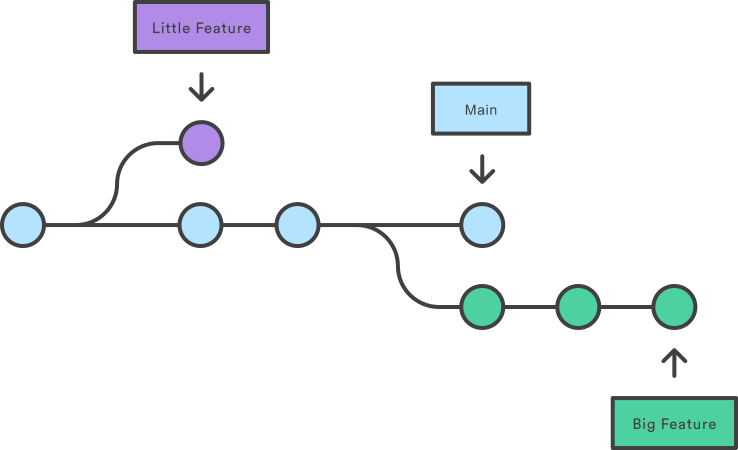
\includegraphics[width=0.5\textwidth]{pictures/01Gitbranch.png}<1>
    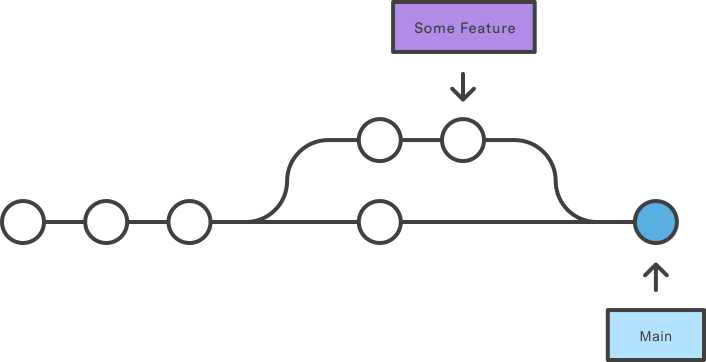
\includegraphics[width=0.5\textwidth]{pictures/05-06Fastforwardmerge.png}<2>
\end{figure}
\end{frame}

\begin{frame}{Branching}
\begin{itemize}
    \item Create a new branch called feature:

        \lstinline{git checkout -b feature} or \lstinline{git switch -c feature}

    \item Get a list of all local branches and of all local and remote branches:

        \lstinline{git branch}
        
        \lstinline{git branch --all}

    \item Create a change, stage, commit and push it. If you still use git command, you will have to add an upstream origin to track the changes when pushing

        \lstinline{git push --set-upstream origin feature}
\end{itemize}
\end{frame}

\begin{frame}{Merging without Conflicts}
Merges into main should be done on GitHub to let other people review changes before merging. For merges from main to your own branches(experimental playgrounds), you can merge locally. But do whatever you like, I am a student, not a GitCop.
\begin{itemize}
    \item Look at your repository on GitHub, you will have two available branches
    \item Create a pull request for your feature branch
    \item Complete the pull request, delete the feature branch when done
    \item Checkout your local main branch. The changes won't be present by now, we still need to:
    
        \lstinline{git pull}
        
        without added upstream: \lstinline{git pull origin main}
    \item git pull will merge changes from the remote into your HEAD. Alternatively, use git fetch to only stage the changes beforehand and only commit what you want
\end{itemize}    
\end{frame}

\begin{frame}{Merging with Conflicts}
When multiple changes happen on the same file, you will have to decide, which changes to keep. This is called resolving a conflict. Let's create and solve a conflict.
\begin{itemize}
    \item Create a new branch slowfeature

        \lstinline{git checkout -b slowfeature}

    \item Make a change in one of the existing files and commit it
    \item Checkout main and do another change in the same file and commit it
    
        \lstinline{git checkout main}

    \item Checkout back to slowfeature, and try to merge main into slowfeature again
    \item Resolve the conflict by deciding on on of the options both or none
    \item Stage and commit the resolved change
    \item Boast about your conflict management skills in your resume 
\end{itemize}    
\end{frame}

\begin{frame}{Other Features on GitHub}
    \begin{itemize}
        \item Displays the README.md to inform other about the purpose of the project/give instructions how to use it
        \item Ability to change files, create/delete branches on the remote
        \item Remark issues in projects
        \item Create pull requests
        \item Configuration of security and requirements for commits
        \item General statistics, including a graph representation of the branches
    \end{itemize}
    
\end{frame}

\begin{frame}{git clone/git fork}
To use other code from GitHub, you will have to clone it and use it locally. Copy the url and use the command \lstinline{git clone THE_URL_GOES_HERE}. You now have a local version of the remote, but you might lack the necessary permissions to actually push changes.

\vspace{12pt}
If you actually want to keep developing on someone else's code, you might want to fork it instead. In the top right corner of the repository on GitHub there is an option to fork the repository. This will copy the repository and create your own repository from it, that you can clone and use as you like.
    
\end{frame}

\begin{frame}{.gitignore}
The .gitignore is a special file inside a git-repository. Any file name inside it will not be tracked by git commands. It allows * as placeholder, with e.g. *.csv any csv files in the will not be affected by commands like \lstinline{git add .}, which would normally stage all changes in the folder. They also won't show up as changed when comparing between different commits. Temporary files or constantly changing files like logs are probably something, that you would add to your .gitignore
    
\end{frame}

\begin{frame}{Summary}
\begin{columns}[t]
\begin{column}{0.45\textwidth}
\begin{block}{Commits}
\lstinline{git add .}\\
\lstinline{git commit -m "..."}\\
\lstinline{git push}
\end{block}
\end{column}

\begin{column}{0.45\textwidth}
\begin{block}{Branching \& Merging}
\lstinline{git checkout -b new_branch}\\
...\\
\lstinline{git checkout main}\\
\lstinline{git merge new_branch}\\
\lstinline{git branch -d new_branch}
\end{block}
\end{column}
\end{columns}
    
\end{frame}

\begin{frame}{Further Information}
    \begin{itemize}
        \item Original documentation(kinda hard to digest): \url{https://git-scm.com/doc}
        \item Nice set of tutorials: \url{https://www.atlassian.com/git/tutorials}
        \item Good explanation: \url{https://www.youtube.com/watch?v=RGOj5yH7evk}
        \item Git for dummies: \url{https://www.youtube.com/watch?v=mJ-qvsxPHpY}
    \end{itemize}
\end{frame}

\begin{frame}{Playground}
    Please let me know your GitHub-Account and experiment around on your own for a while.
    \vspace{12pt}
    
    I'll add you as collaborators to this test-repository. Then try to create branches, merge them, mess stuff up, and clean up other's mistakes.
    \vspace{12pt}
    
    Try to find problems, where you can't do what you want, so that we can go through them together again.
\end{frame}

\end{document}